	\section{Appendix}
	
	\subsection{Mode Hopping}
	\begin{multicols}{2}
		% Mode Hopping
		\begin{figure}[H]
			\centering
			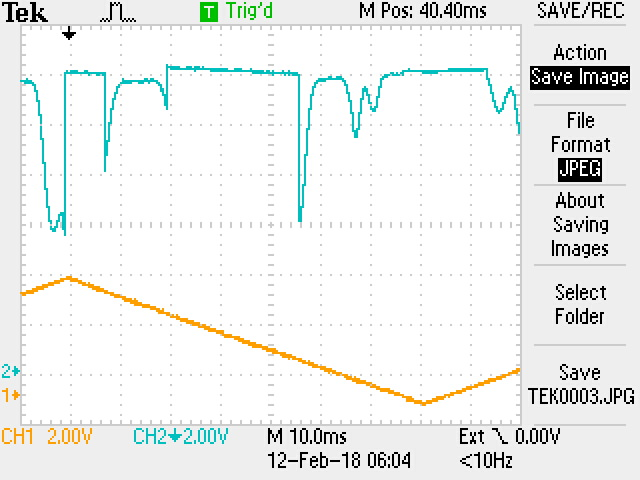
\includegraphics[width=0.4\textwidth]{Oscilloscope/ModeHopping.JPG}
			\caption{Rubidium spectrum with mode hopping}
			\label{modeHopping}
		\end{figure}
	
		\columnbreak
		
		Here, we can see the spectrum of Rubidium with mode hopping, seen as sharp discontinuous jumps in the spectrum.
	\end{multicols}

	The series of graphs below depict mode hopping between the grating feedback and external cavity and internal cavity. We can see that as the relative frequency of the external cavity is increased, the laser hops to the mode with the most overlap. In graphs a-c, the laser hops through grating feedback and external cavity modes, but in d, the laser hops up to the next internal cavity mode. 
	\begin{figure}[H]
		\centering
		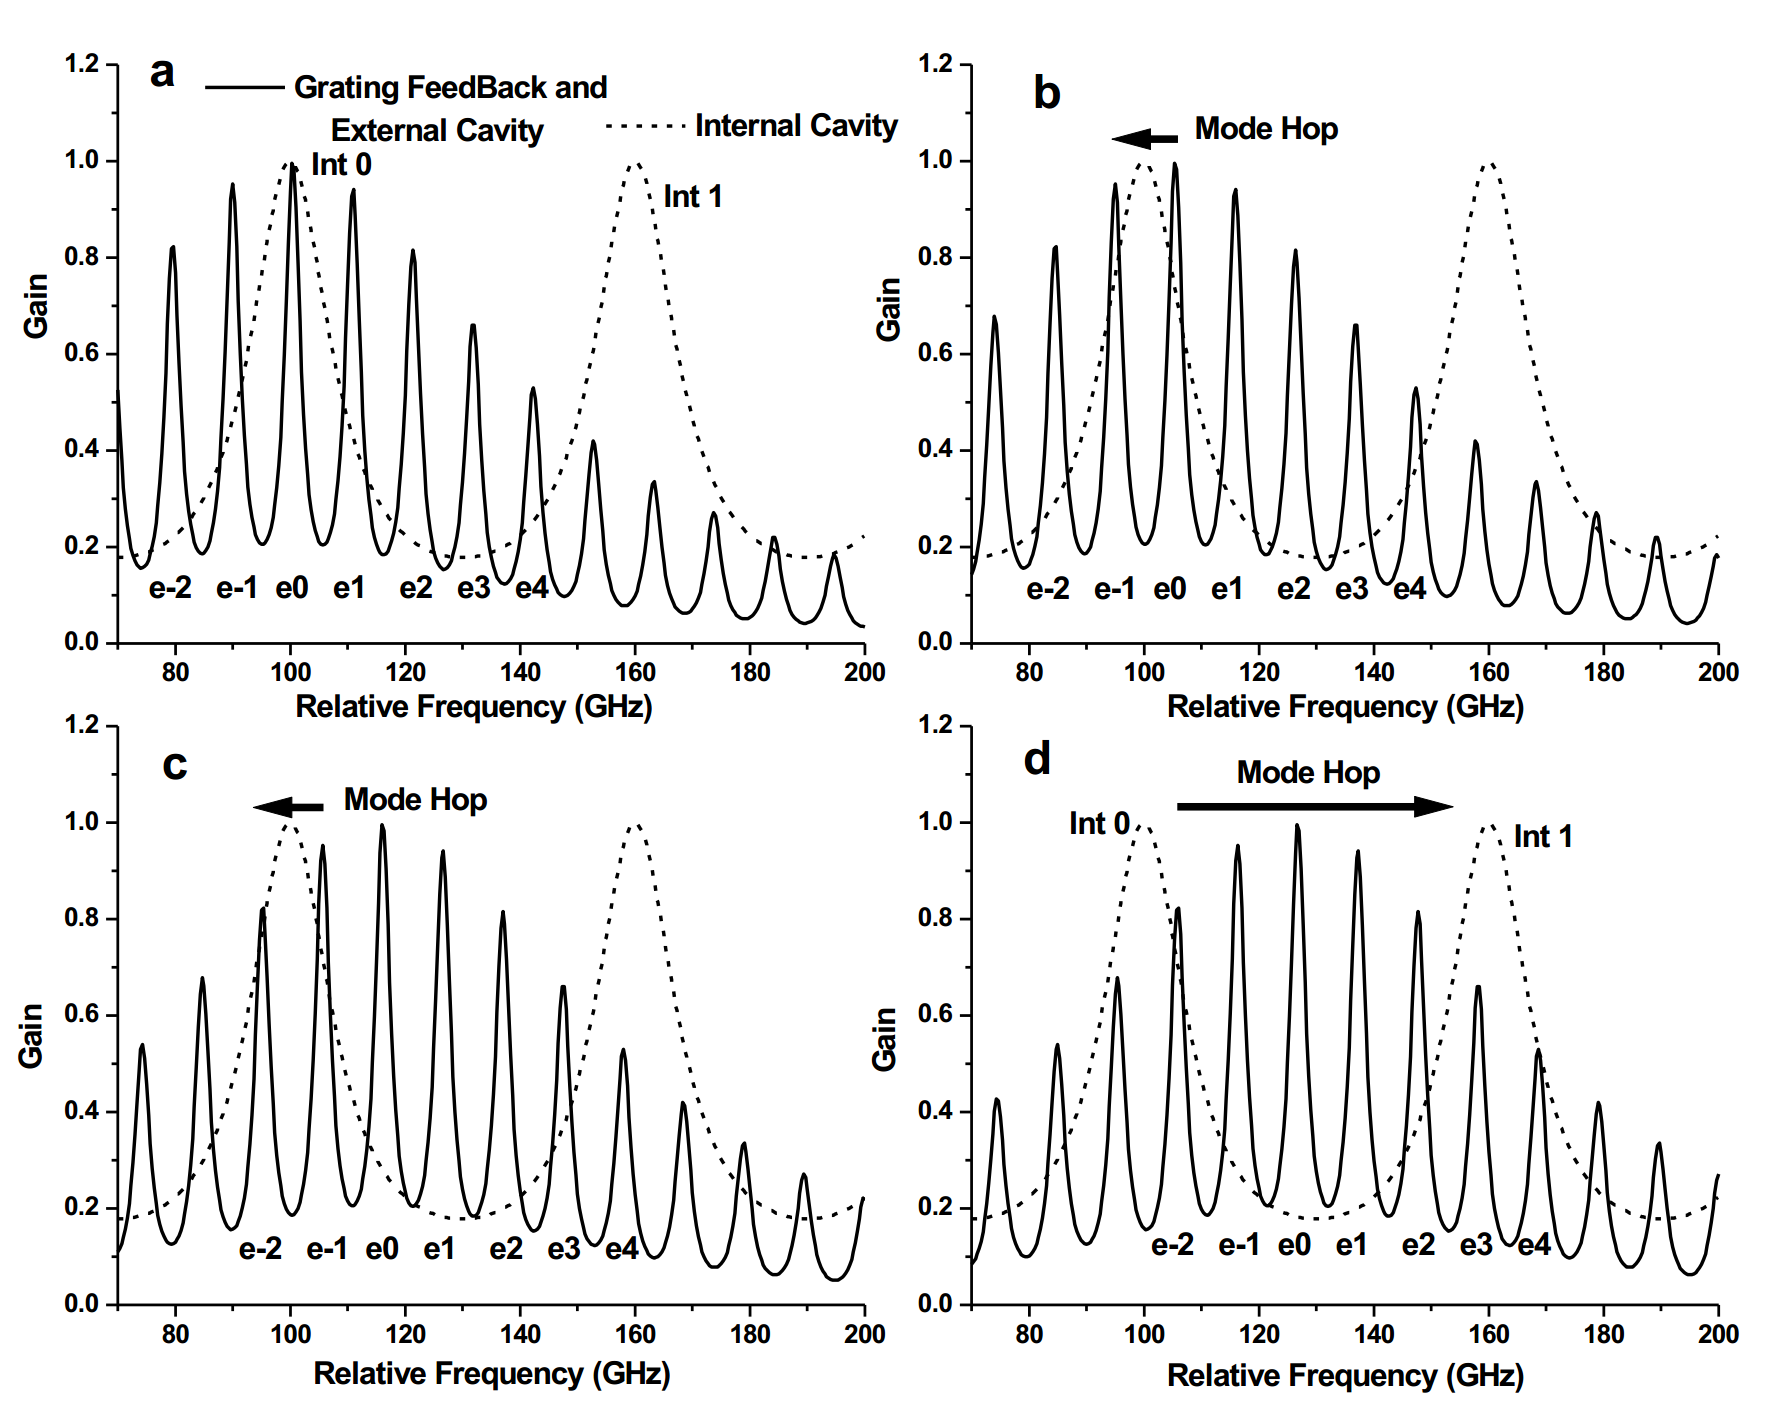
\includegraphics[height=0.4\textheight]{DiodeLaser/modeHops.PNG}
		\caption{Depiction of mode hopping}
		\label{modeHops}
	\end{figure}
	
	\subsection{Zeeman Splitting}
	
	\begin{figure}[H]
		\centering
		\subfloat[$B = 0$ Gauss]
		{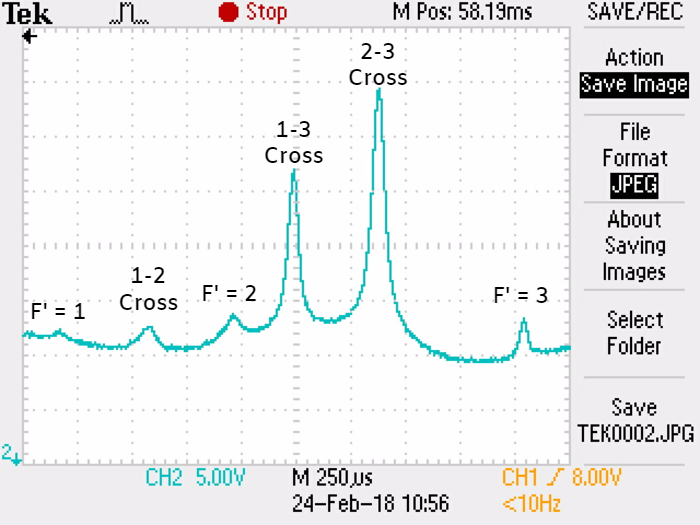
\includegraphics[width=0.3\textwidth]{HyperFineBField/UseThisOne/P10_0AAnnotated.JPG}}
		\qquad
		\subfloat[$B = 16.5$ Gauss]
		{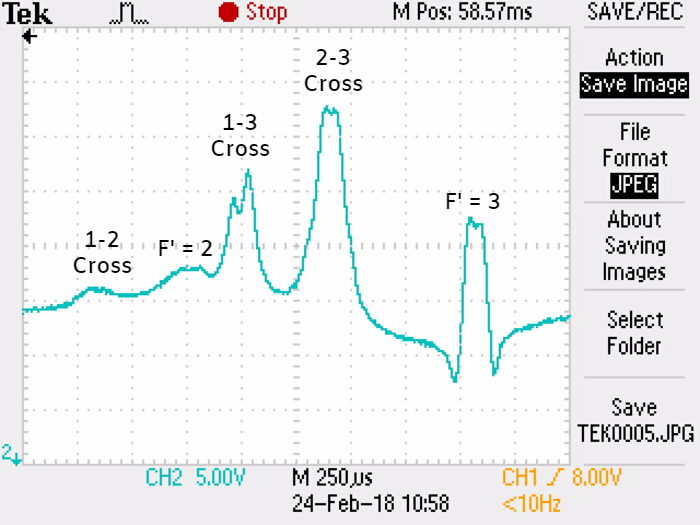
\includegraphics[width=0.3\textwidth]{HyperFineBField/UseThisOne/P10_5AAnnotated.JPG}}
		
		\subfloat[$B = 33.0$ Gauss]
		{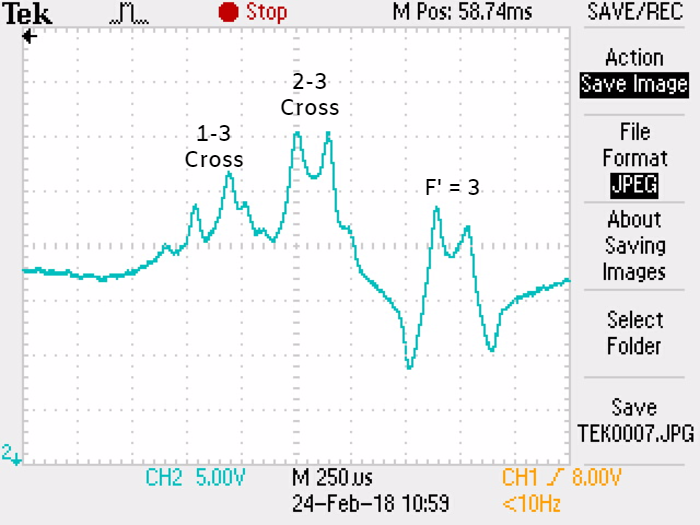
\includegraphics[width=0.3\textwidth]{HyperFineBField/UseThisOne/P11_0AAnnotated.JPG}}
		\qquad
		\subfloat[$B = 49.4$ Gauss]
		{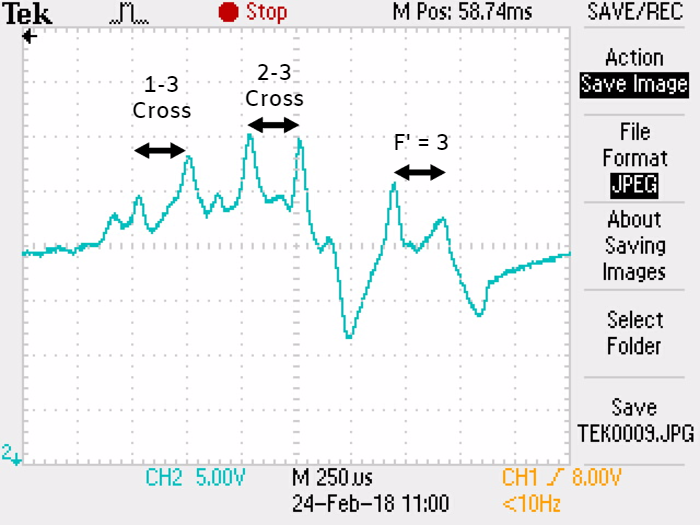
\includegraphics[width=0.3\textwidth]{HyperFineBField/UseThisOne/P11_5AAnnotated.JPG}}
		
		\subfloat[$B = 65.9$ Gauss]
		{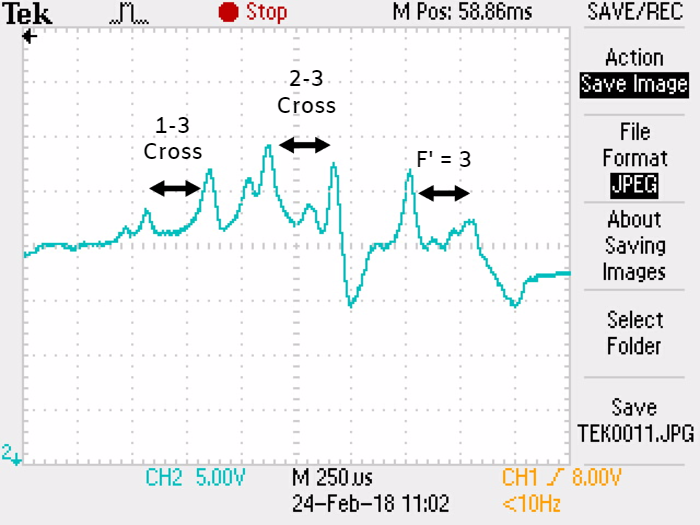
\includegraphics[width=0.3\textwidth]{HyperFineBField/UseThisOne/P12_0AAnnotated.JPG}}
		\qquad
		\subfloat[$B = 82.4$ Gauss]
		{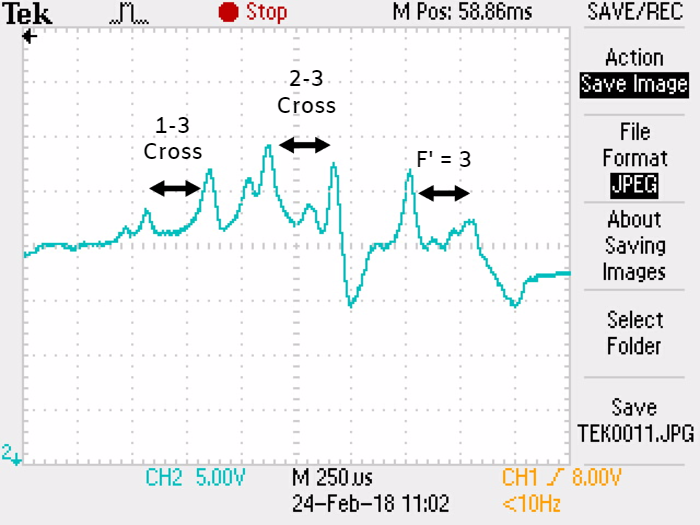
\includegraphics[width=0.3\textwidth]{HyperFineBField/UseThisOne/P12_5AAnnotated.png}}
		
		\subfloat[$B = 98.9$ Gauss]
		{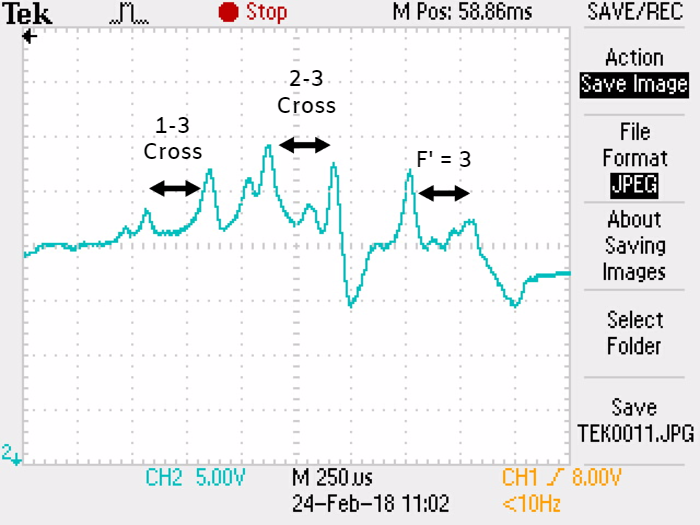
\includegraphics[width=0.3\textwidth]{HyperFineBField/UseThisOne/P13_0AAnnotated.png}}
		
		\caption{\RbES Zeeman splitting of the 1-3 crossover, 2-3 crossover, and $F'=3$ state for various magnetic field strengths.}
		\label{HyperFineBField}
	\end{figure}

%\cref{HyperFineBField} details the Zeeman splitting for the \RbES $\text{F}=2$ peak. 
	
	